% Created by tikzDevice version 0.12.3.1 on 2021-12-06 10:56:48
% !TEX encoding = UTF-8 Unicode
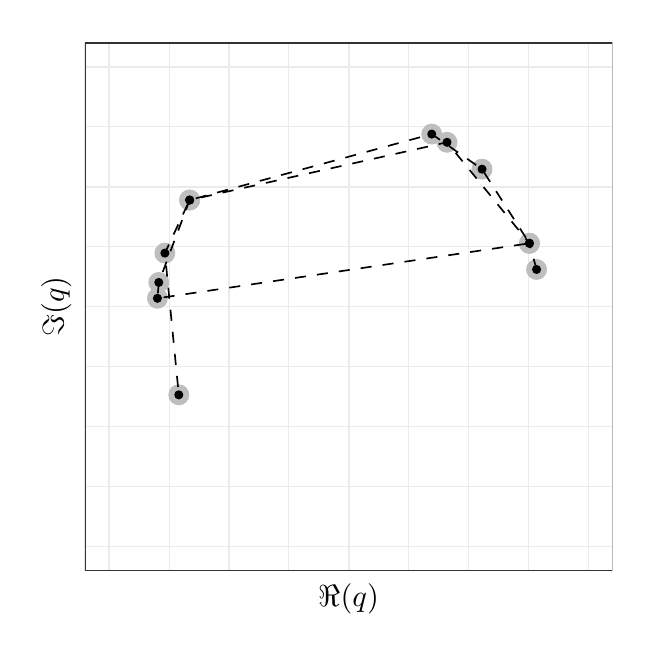
\begin{tikzpicture}[x=1pt,y=1pt]
\definecolor{fillColor}{RGB}{255,255,255}
\path[use as bounding box,fill=fillColor,fill opacity=0.00] (0,0) rectangle (216.81,216.81);
\begin{scope}
\path[clip] (  0.00,  0.00) rectangle (216.81,216.81);
\definecolor{drawColor}{RGB}{255,255,255}
\definecolor{fillColor}{RGB}{255,255,255}

\path[draw=drawColor,line width= 0.6pt,line join=round,line cap=round,fill=fillColor] (  0.00,  0.00) rectangle (216.81,216.81);
\end{scope}
\begin{scope}
\path[clip] ( 20.71, 20.71) rectangle (211.31,211.31);
\definecolor{fillColor}{RGB}{255,255,255}

\path[fill=fillColor] ( 20.71, 20.71) rectangle (211.31,211.31);
\definecolor{drawColor}{gray}{0.92}

\path[draw=drawColor,line width= 0.3pt,line join=round] ( 20.71, 51.04) --
	(211.31, 51.04);

\path[draw=drawColor,line width= 0.3pt,line join=round] ( 20.71, 94.35) --
	(211.31, 94.35);

\path[draw=drawColor,line width= 0.3pt,line join=round] ( 20.71,137.67) --
	(211.31,137.67);

\path[draw=drawColor,line width= 0.3pt,line join=round] ( 20.71,180.99) --
	(211.31,180.99);

\path[draw=drawColor,line width= 0.3pt,line join=round] ( 51.04, 20.71) --
	( 51.04,211.31);

\path[draw=drawColor,line width= 0.3pt,line join=round] ( 94.35, 20.71) --
	( 94.35,211.31);

\path[draw=drawColor,line width= 0.3pt,line join=round] (137.67, 20.71) --
	(137.67,211.31);

\path[draw=drawColor,line width= 0.3pt,line join=round] (180.99, 20.71) --
	(180.99,211.31);

\path[draw=drawColor,line width= 0.6pt,line join=round] ( 20.71, 29.38) --
	(211.31, 29.38);

\path[draw=drawColor,line width= 0.6pt,line join=round] ( 20.71, 72.69) --
	(211.31, 72.69);

\path[draw=drawColor,line width= 0.6pt,line join=round] ( 20.71,116.01) --
	(211.31,116.01);

\path[draw=drawColor,line width= 0.6pt,line join=round] ( 20.71,159.33) --
	(211.31,159.33);

\path[draw=drawColor,line width= 0.6pt,line join=round] ( 20.71,202.65) --
	(211.31,202.65);

\path[draw=drawColor,line width= 0.6pt,line join=round] ( 29.38, 20.71) --
	( 29.38,211.31);

\path[draw=drawColor,line width= 0.6pt,line join=round] ( 72.69, 20.71) --
	( 72.69,211.31);

\path[draw=drawColor,line width= 0.6pt,line join=round] (116.01, 20.71) --
	(116.01,211.31);

\path[draw=drawColor,line width= 0.6pt,line join=round] (159.33, 20.71) --
	(159.33,211.31);

\path[draw=drawColor,line width= 0.6pt,line join=round] (202.65, 20.71) --
	(202.65,211.31);
\definecolor{drawColor}{RGB}{190,190,190}
\definecolor{fillColor}{RGB}{190,190,190}

\path[draw=drawColor,line width= 0.4pt,line join=round,line cap=round,fill=fillColor] (183.89,129.43) circle (  3.57);

\path[draw=drawColor,line width= 0.4pt,line join=round,line cap=round,fill=fillColor] (181.31,138.89) circle (  3.57);

\path[draw=drawColor,line width= 0.4pt,line join=round,line cap=round,fill=fillColor] (151.53,175.39) circle (  3.57);

\path[draw=drawColor,line width= 0.4pt,line join=round,line cap=round,fill=fillColor] ( 58.53,154.52) circle (  3.57);

\path[draw=drawColor,line width= 0.4pt,line join=round,line cap=round,fill=fillColor] ( 47.38,124.75) circle (  3.57);

\path[draw=drawColor,line width= 0.4pt,line join=round,line cap=round,fill=fillColor] ( 46.89,119.02) circle (  3.57);

\path[draw=drawColor,line width= 0.4pt,line join=round,line cap=round,fill=fillColor] (181.31,138.89) circle (  3.57);

\path[draw=drawColor,line width= 0.4pt,line join=round,line cap=round,fill=fillColor] (164.18,165.68) circle (  3.57);

\path[draw=drawColor,line width= 0.4pt,line join=round,line cap=round,fill=fillColor] (146.01,178.36) circle (  3.57);

\path[draw=drawColor,line width= 0.4pt,line join=round,line cap=round,fill=fillColor] ( 58.53,154.52) circle (  3.57);

\path[draw=drawColor,line width= 0.4pt,line join=round,line cap=round,fill=fillColor] ( 49.58,135.35) circle (  3.57);

\path[draw=drawColor,line width= 0.4pt,line join=round,line cap=round,fill=fillColor] ( 54.61, 84.13) circle (  3.57);
\definecolor{drawColor}{RGB}{0,0,0}

\path[draw=drawColor,line width= 0.6pt,dash pattern=on 4pt off 4pt ,line join=round] (183.89,129.43) --
	(181.31,138.89) --
	(151.53,175.39) --
	( 58.53,154.52) --
	( 47.38,124.75) --
	( 46.89,119.02) --
	(181.31,138.89) --
	(164.18,165.68) --
	(146.01,178.36) --
	( 58.53,154.52) --
	( 49.58,135.35) --
	( 54.61, 84.13);
\definecolor{fillColor}{RGB}{0,0,0}

\path[draw=drawColor,line width= 0.4pt,line join=round,line cap=round,fill=fillColor] (183.89,129.43) circle (  1.43);

\path[draw=drawColor,line width= 0.4pt,line join=round,line cap=round,fill=fillColor] (181.31,138.89) circle (  1.43);

\path[draw=drawColor,line width= 0.4pt,line join=round,line cap=round,fill=fillColor] (151.53,175.39) circle (  1.43);

\path[draw=drawColor,line width= 0.4pt,line join=round,line cap=round,fill=fillColor] ( 58.53,154.52) circle (  1.43);

\path[draw=drawColor,line width= 0.4pt,line join=round,line cap=round,fill=fillColor] ( 47.38,124.75) circle (  1.43);

\path[draw=drawColor,line width= 0.4pt,line join=round,line cap=round,fill=fillColor] ( 46.89,119.02) circle (  1.43);

\path[draw=drawColor,line width= 0.4pt,line join=round,line cap=round,fill=fillColor] (181.31,138.89) circle (  1.43);

\path[draw=drawColor,line width= 0.4pt,line join=round,line cap=round,fill=fillColor] (164.18,165.68) circle (  1.43);

\path[draw=drawColor,line width= 0.4pt,line join=round,line cap=round,fill=fillColor] (146.01,178.36) circle (  1.43);

\path[draw=drawColor,line width= 0.4pt,line join=round,line cap=round,fill=fillColor] ( 58.53,154.52) circle (  1.43);

\path[draw=drawColor,line width= 0.4pt,line join=round,line cap=round,fill=fillColor] ( 49.58,135.35) circle (  1.43);

\path[draw=drawColor,line width= 0.4pt,line join=round,line cap=round,fill=fillColor] ( 54.61, 84.13) circle (  1.43);
\definecolor{drawColor}{gray}{0.20}

\path[draw=drawColor,line width= 0.6pt,line join=round,line cap=round] ( 20.71, 20.71) rectangle (211.31,211.31);
\end{scope}
\begin{scope}
\path[clip] (  0.00,  0.00) rectangle (216.81,216.81);
\definecolor{drawColor}{RGB}{0,0,0}

\node[text=drawColor,anchor=base,inner sep=0pt, outer sep=0pt, scale=  1.10] at (116.01,  7.64) {$\Re(q)$};
\end{scope}
\begin{scope}
\path[clip] (  0.00,  0.00) rectangle (216.81,216.81);
\definecolor{drawColor}{RGB}{0,0,0}

\node[text=drawColor,rotate= 90.00,anchor=base,inner sep=0pt, outer sep=0pt, scale=  1.10] at ( 13.08,116.01) {$\Im(q)$};
\end{scope}
\end{tikzpicture}
